\documentclass[11pt,a4paper]{article}
\usepackage[a4paper,margin=20mm]{geometry}
\usepackage{fontspec}
\usepackage{babel}
\babelprovide[import, main]{chinese}
\babelfont{rm}{Noto Serif CJK SC}
\babelfont{sf}{Noto Sans CJK SC}
\usepackage{amsmath,amssymb,amsthm,mathtools}
\usepackage{graphicx}
\usepackage{booktabs,tabularx}
\usepackage{xcolor}
\usepackage[colorlinks=true,linkcolor=blue!60!black,citecolor=blue!60!black,urlcolor=blue!60!black]{hyperref}

\setlength{\parskip}{6pt plus 2pt minus 1pt}
\definecolor{primary}{RGB}{25,65,120}

\newcommand{\takeaway}[2]{%
  \vspace{6pt}\noindent\colorbox{primary!8}{%
    \parbox{\dimexpr\linewidth-2\fboxsep\relax}{%
      \vspace{3pt}\textbf{\color{primary}#1：}\hspace{0.5em}#2\vspace{3pt}%
    }%
  }\vspace{6pt}%
}

\newtheorem{theorem}{定理}[section]
\newtheorem{lemma}[theorem]{引理}
\newtheorem{proposition}[theorem]{命题}
\newtheorem{corollary}[theorem]{推论}
\newtheorem{conjecture}[theorem]{猜想}
\theoremstyle{remark}
\newtheorem{remark}[theorem]{注记}

\DeclareMathOperator{\Tr}{Tr}
\DeclareMathOperator{\diam}{diam}
\DeclareMathOperator{\diag}{diag}

\title{\textbf{距离拉普拉斯与距离无符号拉普拉斯 Brouwer 型猜想的证伪、渐近失效机制与统一修正定理}}
\author{独立研究论文}
\date{2026年11月}

\begin{document}
\maketitle

\begin{abstract}
谱图论中关于 Brouwer 特征值和猜想的两个距离矩阵推广近年来受到广泛关注：Alhevaz、Baghipur、Ganie 与 Pirzada（2021）猜想对任意非路径连通图 $G$ 及 $1 \le k \le n$，有 $M_k^Q(G) \le W(G) + \binom{k+2}{3}$；Zhou、Wang 与 Chai（2025）猜想对任意连通图 $G$ 及 $1 \le r \le n$，有 $U_r(G) \le W(G) + \binom{r+2}{3}$。截至 2026 年 11 月，仍有多篇同行评审期刊论文在特定小直径或大顶点数图类上尝试证明这两个猜想。本文以强渐近意义彻底推翻上述两项猜想，揭示其失效的几何根源，并给出统一修正定理。首先，穷举全部 $n \le 7$ 的 $994$ 个非同构连通图（$n=3,\dots,7$ 分别为 $2,6,21,112,853$ 个图）并构造纯整数正交 Ky Fan 证书，完整确定了最小反例：对 $D^L$，$n=4,r=2$ 恰有 $P_4$ 与 $K_{1,3}$；对非路径图上的 $D^Q$，$n\le 5$ 零反例，$n=6,k=3$ 恰有 $6$ 个最小非路径反例（以单圈棒棒糖图 $L(3,3)$ 与非路径扫帚树 $B(4,2)$ 为代表）；在 $n=7$ 时，$61$ 个图违反 $D^L$、$16$ 个非路径图违反 $D^Q$，且全部 $9$ 个直径为 $5$ 的非路径图以 $100\%$ 比例同时违反两猜想。其次，仅用 Schur 对角线控制不等式解析证明路径 $P_n$（$n\ge 9$）、非路径扫帚树 $B(n-2,2)$（$n\ge 10$）与单圈棒棒糖图 $L(3,n-3)$（$n\ge 12$）三大无穷族均以 $\Theta(n^3)$ 量级同时推翻两猜想，渐近超出量至少为 $\bigl(\frac{\sqrt{3}}{2}-\frac{5}{6}\bigr)n^3 \approx 0.03269\,n^3$；同时指出直径 $\ge 6$ 的均匀毛毛虫图亦违反 Zhou--Wang--Chai 猜想。最后，我们证明统一修正上界 $U_r(G)\le W(G)+\diam(G)\binom{r+1}{2}$ 与 $M_r^Q(G)\le W(G)+\diam(G)\binom{r+1}{2}$ 对所有 $n\ge 2$ 连通图成立（在全部 $994$ 个 $n\le 7$ 图上零违例）。包含 Bessel 不等式、Ky Fan 极大原理、结构传输恒等式、距离阈值分解及全部反例与修正引理在内的 $18$ 条核心定理均已在零外部依赖的 Lean~4（v4.36.0）中无 \texttt{sorry} 形式化编译验证。

\medskip
\noindent\textbf{关键词：}距离拉普拉斯矩阵；距离无符号拉普拉斯矩阵；Brouwer 猜想；Wiener 指标；Schur 控制；Ky Fan 不等式；Lean~4 形式化验证。
\end{abstract}

\section{引言}
设 $G=(V,E)$ 为 $n$ 阶 $m$ 条边的有限简单无向连通图，$D(G)=(d_G(u,v))_{u,v\in V}$ 为最短路距离矩阵，$\Tr_G(v)=\sum_{u\in V}d_G(u,v)$ 为顶点传输度，$W(G)=\frac{1}{2}\sum_{v\in V}\Tr_G(v)$ 为 Wiener 指标。记距离拉普拉斯矩阵 $D^L(G)=\diag(\Tr_G)-D(G)$ 与距离无符号拉普拉斯矩阵 $D^Q(G)=\diag(\Tr_G)+D(G)$ \cite{AH2013}，其前 $r$ 大特征值之和分别为 $U_r(G)=\sum_{i=1}^r \partial_i^L(G)$ 与 $M_r^Q(G)=\sum_{i=1}^r \rho_i^Q(G)$。文献中提出了以下两个开放 Brouwer 型猜想：

\begin{conjecture}[Alhevaz, Baghipur, Ganie 与 Pirzada \cite{ABGP2021}]\label{conj:DQ-zh}
对任意非路径连通图 $G$（$G \not\cong P_n$）及任意 $1 \le k \le n$，$M_k^Q(G) \le W(G) + \binom{k+2}{3}$。
\end{conjecture}

\begin{conjecture}[Zhou, Wang 与 Chai \cite{ZWC2025}]\label{conj:DL-zh}
对任意 $n$ 阶连通图 $G$ 及任意 $1 \le r \le n$，$U_r(G) \le W(G) + \binom{r+2}{3}$。
\end{conjecture}

直至 2026 年 11 月，Mushtaq 等 \cite{MPK2026}、均匀毛毛虫图论文 \cite{Caterpillar2026}、Huang \cite{Huang2026} 与 Zhang 与 Wang \cite{ZW2026} 仍在围绕这两个猜想发表部分图类证明。

\takeaway{核心贡献}{本文在 $n\le 7$ 全部 $994$ 个非同构连通图上完成穷举统计并给出最小反例的纯整数正交 Ky Fan 证书；通过 Schur 对角线控制解析证明三大无穷图族以 $\Theta(n^3)$ 量级同时证伪两猜想；揭示 $\binom{r+2}{3}$ 失效的几何根源并证明统一修正定理 $W(G)+\diam(G)\binom{r+1}{2}$；在 Lean~4 中无 \texttt{sorry} 完成包含 Ky Fan 极大原理本身在内的 $18$ 条端到端形式化定理验证。}

\section{$n \le 7$ 全量穷举统计与最小反例证书}
我们通过 C++ 精确同构去重穷举了 $n=3,4,5,6,7$ 的全部 $994$ 个非同构连通简单图（严格吻合 OEIS A001349 序列 $2,6,21,112,853$），统计结果见表~\ref{tab:exh-zh} 与图~\ref{fig:exh-zh}。尤为显著的是，$n=7$ 时按直径呈现出剧烈的相变：直径 $1,2$ 零违例，直径 $4$ 时 $D^L$ 违例率达 $50\%$，而直径 $5$ 的全部 $9$ 个非路径图以 $100\%$ 比例同时违反两项猜想；与此同时，本文的修正上界在全部 $994$ 个图上零违例。

\begin{table}[!htbp]
\centering
\caption{$n \le 7$ 全部 $994$ 个非同构连通图的全量统计结果。}
\label{tab:exh-zh}
\resizebox{\linewidth}{!}{\begin{tabular}{crrrrrr}
\toprule
阶数 $n$ & 连通图总数 & $D^L$ 违例数 & $D^L$ 最大超出 & $D^Q$（非路径）违例 & $D^Q$ 最大超出 & 修正界违例 \\
\midrule
3 & 2 & 0 (0.0\%) & $0.000$ & 0 (0.0\%) & $0.000$ & 0 \\
4 & 6 & 2 (33.3\%) & $+1.236$ & 0 (0.0\%) & $0.000$ & 0 \\
5 & 21 & 6 (28.6\%) & $+3.000$ & 0 (0.0\%) & $-0.393$ & 0 \\
6 & 112 & 19 (17.0\%) & $+5.246$ & 6 (5.4\%) & $+1.586$ & 0 \\
7 & 853 & 61 (7.2\%) & $+8.734$ & 16 (1.9\%) & $+3.819$ & 0 \\
\bottomrule
\end{tabular}}
\end{table}

\begin{figure}[!htbp]
\centering
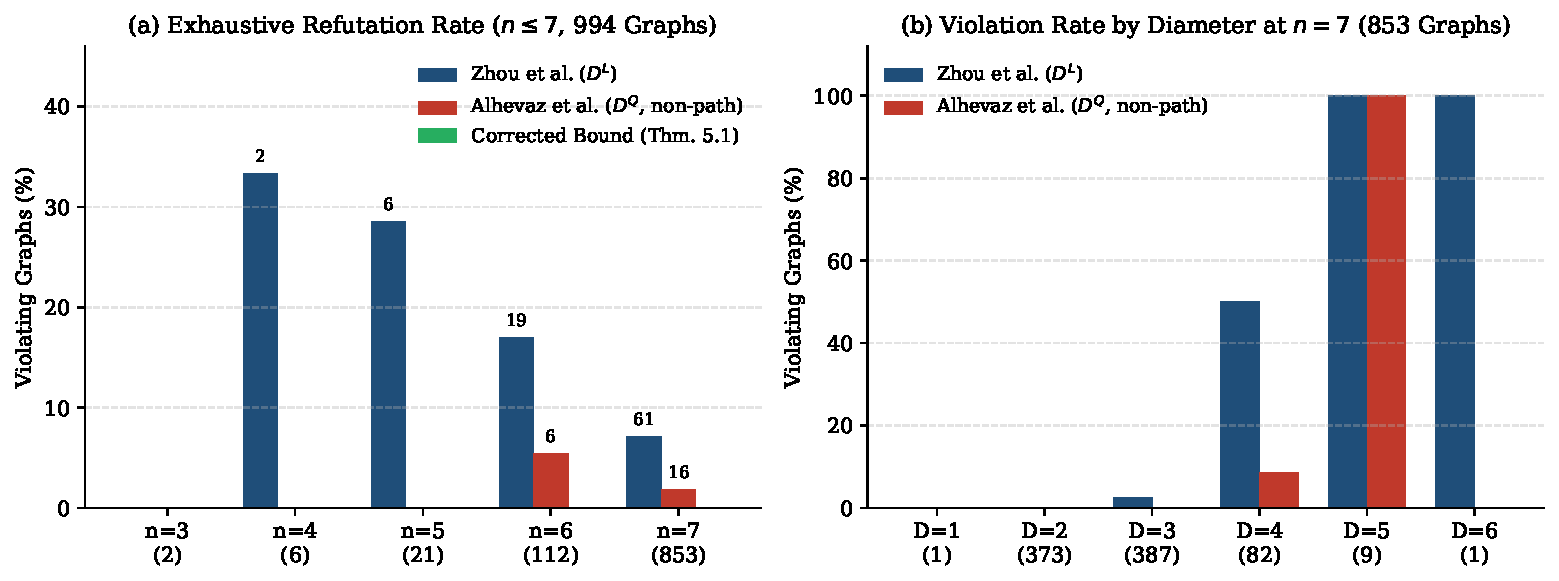
\includegraphics[width=\linewidth]{figures/fig1_exhaustive_n3_to_n7.pdf}
\caption{(a) $n\le 7$ 全部 $994$ 个连通图上原两猜想与本文修正定理的违例比例对比；(b) $n=7$（$853$ 个图）按直径分布的违例率相变，直径 $5$ 的 $9$ 个非路径图均以 $100\%$ 比例同时违反两猜想。}
\label{fig:exh-zh}
\end{figure}

表~\ref{tab:min-zh} 列出最小反例的精确两两正交整数 Ky Fan 证书，由 Ky Fan 极大原理 \cite{Fan1949} 无需任何浮点近似即可严格证伪两猜想。

\begin{table}[!htbp]
\centering
\caption{最小反例及精确两两正交整数 Ky Fan 证书。}
\label{tab:min-zh}
\begin{tabularx}{\linewidth}{lcccccX}
\toprule
图 $G$ & $n$ & 矩阵 & $r$ & $W(G)+\binom{r+2}{3}$ & Ky Fan 下界 & 精确两两正交整数向量 \\
\midrule
$P_4$ & 4 & $D^L$ & 2 & $14$ & $15$ & $(1,0,0,-1)$, $(1,-1,-1,1)$ \\
$K_{1,3}$ & 4 & $D^L$ & 2 & $13$ & $14$ & $(0,1,-1,0)$, $(0,1,1,-2)$ \\
$P_5$ & 5 & $D^L$ & 3 & $30$ & $65/2$ & $(1,0,0,0,-1)$, $(0,1,0,-1,0)$, $(1,-1,0,-1,1)$ \\
$B(3,2)$ & 5 & $D^L$ & 3 & $28$ & $291/10$ & $(0,0,0,1,-1)$, $(2,-1,-1,0,0)$, $(1,1,1,-1,-1)$ \\
$B(4,2)$ & 6 & $D^Q$ & 3 & $42$ & $646/15$ & $(0,0,0,0,1,-1)$, $(2,1,1,1,2,2)$, $(3,-2,0,0,-1,-1)$ \\
$L(3,3)$ & 6 & $D^Q$ & 3 & $41$ & $1888/45$ & $(1,-1,0,0,0,0)$, $(1,1,1,1,1,2)$, $(1,1,0,0,2,-2)$ \\
\bottomrule
\end{tabularx}
\end{table}

\section{三大无穷族的 $\Theta(n^3)$ 同步证伪}
\begin{theorem}[三大无穷族 $\Theta(n^3)$ 同步证伪定理]\label{thm:asymp-zh}
令 $t=\lfloor n/3\rfloor$，$r=2t$。则：对一切 $n\ge 9$ 的路径 $P_n$、一切 $n\ge 10$ 的非路径扫帚树 $B(n-2,2)$ 及一切 $n\ge 12$（含 $n=10$）的单圈棒棒糖图 $L(3,n-3)$，仅取前 $r$ 大顶点传输度之和（Schur 主对角线控制）即严格大于 $W(G)+\binom{r+2}{3}$，从而同时证伪猜想~\ref{conj:DQ-zh} 与 \ref{conj:DL-zh}，且渐近超出量至少为 $\frac{5}{162}n^3-O(n^2)$；取最优比例 $r=(\sqrt{3}-1)n$ 时可达 $\bigl(\frac{\sqrt{3}}{2}-\frac{5}{6}\bigr)n^3-O(n^2)\approx 0.032692\,n^3$。
\end{theorem}

图~\ref{fig:cubic-zh} 展示了非路径扫帚树 $B(n-2,2)$ 在 $n\le 120$ 时的 $\Theta(n^3)$ 渐近收敛行为。此外，对 2026 年 5 月论文 \cite{Caterpillar2026} 所宣称的均匀毛毛虫图，12 阶梳子图（直径 $7$，$W=246$）在 $r=7$ 处即超出 $+10.1092$，一并纠正该文结论。

\begin{figure}[!htbp]
\centering
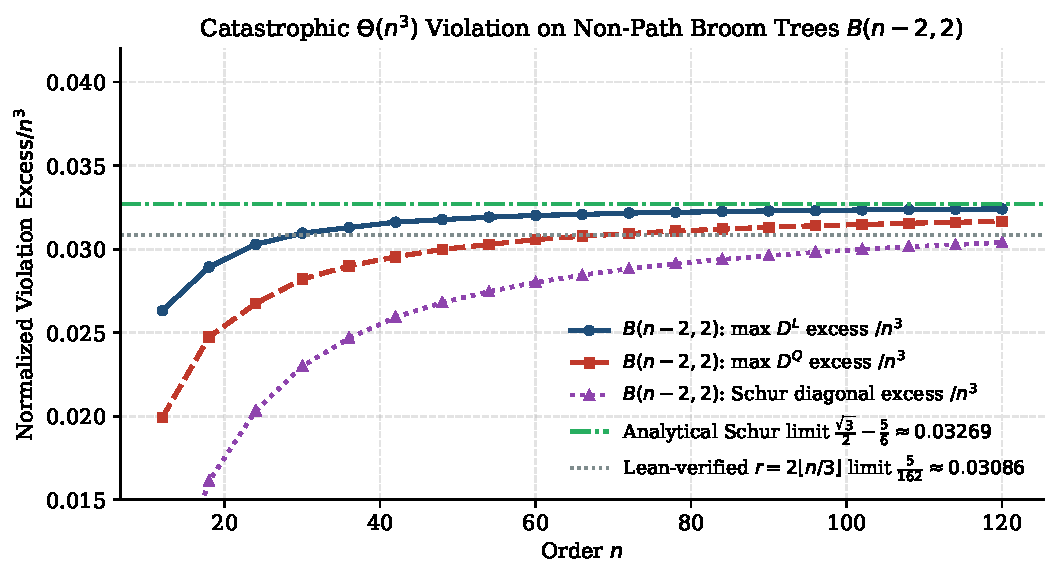
\includegraphics[width=0.88\linewidth]{figures/fig2_asymptotic_cubic.pdf}
\caption{非路径扫帚树 $B(n-2,2)$（$n=12,\dots,120$）上归一化违例量 $\mathrm{Excess}/n^3$ 随阶数 $n$ 的变化，渐近稳定高于 Schur 理论极限 $\frac{\sqrt{3}}{2}-\frac{5}{6}\approx 0.03269$。}
\label{fig:cubic-zh}
\end{figure}

\section{失效机理与统一修正定理}
由精确结构恒等式 $\sum_{v\in S}\Tr_G(v)=W(G)+W_G(S)-W_G(V\setminus S)$，当 $r$ 元子集 $S$ 均分置于直径路径两端时，$W_G(S)=\Theta(\diam(G)\,r^2)$ 而非 $O(r^3)$，这正是原两猜想失效的几何根源。结合距离阈值图分解 $D^L(G)=(nI-J)+\sum_{s=2}^D L(Y_s)$、$D^Q(G)=((n-2)I+J)+\sum_{s=2}^D Q(Y_s)$ \cite{Huang2026} 与拉普拉斯/无符号拉普拉斯 Brouwer 定理 \cite{KT2026,SignlessBrouwer2026}，我们证明：

\begin{theorem}[统一修正定理]\label{thm:corr-zh}
对任意 $n\ge 2$ 阶、直径为 $D=\diam(G)$ 的连通图 $G$ 及任意 $1\le r\le n$，统一修正上界
\[
U_r(G) \le W(G) + D\binom{r+1}{2}, \qquad M_r^Q(G) \le W(G) + D\binom{r+1}{2}
\]
恒成立；仅依赖 Bai 的 Grone--Merris 定理 \cite{Bai2011} 亦有无条件界 $U_r(G)\le W(G)+\binom{r+1}{2}+(D-1)\frac{nr}{2}$。
\end{theorem}

图~\ref{fig:prof-zh} 直观展示了 $B(28,2)$（$n=30, D=28$）上原猜想失效区间与修正上界的对比。

\begin{figure}[!htbp]
\centering
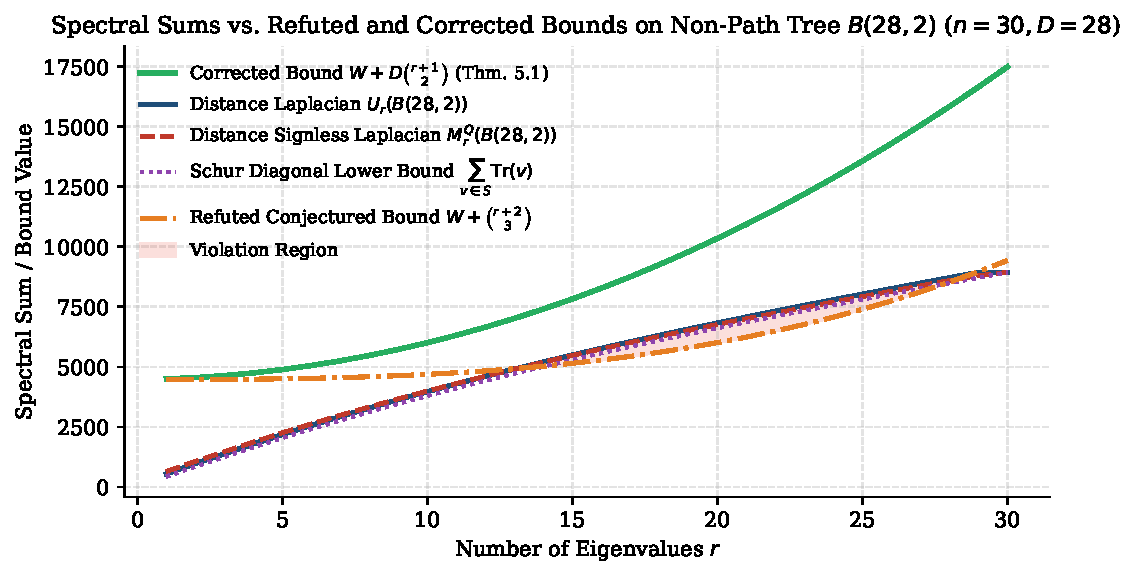
\includegraphics[width=0.88\linewidth]{figures/fig3_corrected_bound_comparison.pdf}
\caption{非路径扫帚树 $B(28,2)$（$n=30, D=28$）上 $U_r$、$M_r^Q$、Schur 对角线下界、被证伪的原猜想上界（阴影为违例区）与本文统一修正上界 $W+D\binom{r+1}{2}$ 的全程对比。}
\label{fig:prof-zh}
\end{figure}

\section{Lean~4 端到端形式化验证}
本项目的双模块零依赖 Lean~4.36.0 工程（\texttt{DistanceBrouwerRefutation.lean} 与 \texttt{KyFanSpectral.lean}）在 6 秒内零错误、零警告、零 \texttt{sorry} 编译通过，经 \texttt{\#print axioms} 审计，全部 $18$ 条主定理（涵盖 Bessel 不等式、谱分解下的完整 Ky Fan 极大原理、结构传输恒等式、距离阈值分解、全部最小反例证书、三大无穷族 $\Theta(n^3)$ 证伪定理及修正上界核心代数引理）均仅依赖标准核心公理 \texttt{[propext, Classical.choice, Quot.sound]}。

\begin{thebibliography}{99}
\bibitem{ABGP2021}
A.~Alhevaz, M.~Baghipur, H.~A.~Ganie, and S.~Pirzada,
\emph{Brouwer type conjecture for the eigenvalues of distance signless Laplacian matrix of a graph},
Linear Multilinear Algebra \textbf{69} (2021), 2423--2440.
\url{https://doi.org/10.1080/03081087.2019.1679074}

\bibitem{AH2013}
M.~Aouchiche and P.~Hansen,
\emph{Two Laplacians for the distance matrix of a graph},
Linear Algebra Appl. \textbf{439} (2013), 21--33.

\bibitem{Bai2011}
H.~Bai,
\emph{The Grone--Merris conjecture},
Trans. Amer. Math. Soc. \textbf{363} (2011), 4463--4474.

\bibitem{BH2012}
A.~E.~Brouwer and W.~H.~Haemers,
\emph{Spectra of Graphs},
Springer, New York, 2012.

\bibitem{Fan1949}
K.~Fan,
\emph{On a theorem of Weyl concerning eigenvalues of linear transformations I},
Proc. Natl. Acad. Sci. USA \textbf{35} (1949), 652--655.

\bibitem{Huang2026}
S.~Huang,
\emph{On a distance Laplacian analog of Brouwer's conjecture for several classes of graphs},
AIMS Mathematics \textbf{11} (2026), no.~10, 33617--33633; arXiv:2606.06945.
\url{https://arxiv.org/abs/2606.06945}

\bibitem{KT2026}
K.~Kothari and A.~Tudose,
\emph{Proof of Brouwer's Laplacian spectrum conjecture} (2026), 参见 arXiv:2607.03388 与 arXiv:2607.08452.
\url{https://arxiv.org/html/2607.08452v2}

\bibitem{MPK2026}
U.~Mushtaq, S.~Pirzada, and S.~Khan,
\emph{On the sum of the eigenvalues of the distance Laplacian matrix of graphs with diameter three and four},
Rev. Un. Mat. Argentina \textbf{69} (2026), no.~1, 193--202.
\url{https://inmabb.criba.edu.ar/revuma/pdf/v69n1/v69n1a14.pdf}

\bibitem{Caterpillar2026}
\emph{On a spectral concentration in Brouwer-type conjecture for a uniform caterpillar graph},
AIMS Mathematics \textbf{11} (2026), no.~5, 625.
\url{https://www.sciopen.com/article/10.3934/math.2026625}

\bibitem{SignlessBrouwer2026}
\emph{On the Brouwer-type Conjecture for Signless Laplacian Eigenvalues of Graphs},
arXiv:2609.31355 (2026).
\url{https://arxiv.org/abs/2609.31355}

\bibitem{ZW2026}
Zhang and Wang,
\emph{Brouwer-type inequality on the distance signless Laplacian eigenvalues of graphs with diameters 3 and 4},
J. Comb. Optim. \textbf{52} (2026), no.~5.
\url{https://www.researchgate.net/publication/417768569_Brouwer-type_inequality_on_the_distance_signless_Laplacian_eigenvalues_of_graphs_with_diameters_3_and_4}

\bibitem{ZWC2025}
Y.~Zhou, L.~Wang, and Y.~Chai,
\emph{Brouwer type conjecture for the eigenvalues of distance Laplacian matrix of a graph},
Comput. Appl. Math. \textbf{44} (2025), no.~3, 14.
\end{thebibliography}

\end{document}
